\documentclass[dvipdfmx]{jsarticle}

\usepackage[version=3]{mhchem}
\usepackage{amsmath}
\usepackage[siunitx]{circuitikz}
\usepackage{graphicx}
\usepackage{here}

\setlength\parindent{0pt}

\begin{document}
\title{情報通信工学レポート}
\author{工学部電子情報工学科3年 03190449  堀 紡希}
\date{\ 10月3日}
\maketitle

\section*{レポート課題1}

図1の三角波は奇関数なのでsin成分のみを持つ。

その成分は、
\begin{align*}
C_{n} &= \int _{-T_{0}/2} ^{T_{0}/2} f(t)\sin{\frac{2\pi }{T_{0}}nt dt}\\
&= \int _{-T_{0}/4}^{-T_{0}/2} \left(-\frac{4}{T_{0}}t-2\right)\sin{\frac{2\pi }{T_{0}}nt dt}
+ \int _{-T_{0}/4}^{T_{0}/4} \frac{4}{T_{0}}t\sin{\frac{2\pi }{T_{0}}nt dt}
+ \int _{-T_{0}/4}^{T_{0}/2} \left(-\frac{4}{T_{0}}+2\right)\sin{\frac{2\pi }{T_{0}}nt dt}\\
&= \left( \frac{T_{0}}{2n\pi}\cos{\frac{n\pi}{2}}+\frac{T_{0}}{(n\pi)^{2}}\sin{\frac{n\pi}{2}} \right) + \left(-\frac{T_{0}}{n\pi}\cos{\frac{n\pi}{2}}+\frac{2T_{0}}{(n\pi)^{2}}\sin{\frac{n\pi}{2}}\right) + \left(\frac{T_{0}}{2n\pi}\cos{\frac{n\pi}{2}}-\frac{T_{0}}{(n\pi)^{2}}\sin{\frac{n\pi}{2}}\right)\\
&= \frac{2T_{0}}{(n\pi)^{2}}\sin{\frac{n\pi}{2}}
\end{align*}

となる。
\section*{レポート課題2}
\subsection*{1.}

(a)のフーリエ変換は、$f\neq \pm f_{0}$のとき、
\begin{align*}
\int _{-\infty } ^{\infty } A\cos{(2\pi ft)} e^{-j\omega t}dt&= \frac{A}{2}\int _{-\frac{T}{2} } ^{\frac{T}{2} } (e^{j2\pi f_{0}t}+e^{-j2\pi f_{0}t}) e^{-j 2\pi f t}dt \\
&= \frac{A}{2}\int _{-\frac{T}{2} } ^{\frac{T}{2} } (e^{j2\pi (-f+f_{0})t}+e^{-j2\pi (f+f_{0})t})dt \\
&= \frac{A}{2}\left[ \frac{e^{j2\pi (-f+f_{0})t}}{j2\pi (-f+f_{0})}+\frac{e^{-j2\pi (f-f_{0})t}}{-j2\pi (f-f_{0})} \right]^{\frac{T}{2}} _{-\frac{T}{2}}\\
&=\frac{A}{2\pi}\left( \frac{\sin{\pi (f+f_{0})T}}{f+f_{0}} + \frac{\sin{\pi (f-f_{0})T}}{f-f_{0}}\right)
\end{align*}

である。($f=\pm f_{0}$でも問題なく成り立つ)
\begin{center}
\begin{figure}[H]
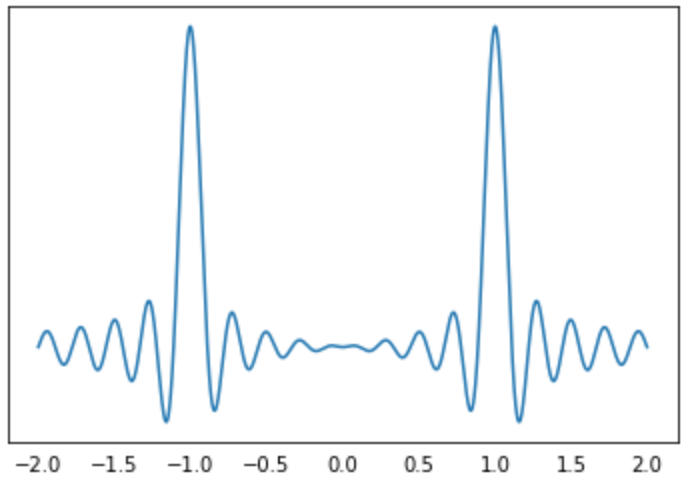
\includegraphics[scale = 1]{2_1.png}
\caption{(a)のスペクトル}
\end{figure}
\end{center}

\subsection*{2.}

(b)のフーリエ変換は、
\begin{align*}
\int _{-\frac{T}{2}} ^{\frac{T}{2}} \frac{2}{T} t e^{-j2\pi ft}dt &=\left[ \frac{\frac{2}{T}te^{-j2\pi f t}}{-j2\pi f}\right]^{\frac{T}{2}}_{-\frac{T}{2}} + \int ^{\frac{T}{2}} _{-\frac{T}{2}} \frac{2e^{-j2\pi ft}}{j2\pi fT}dt\\
&=\frac{j\cos{\pi fT}}{\pi f} + \frac{2}{(2\pi f)^{2}T}\left( e^{-j\pi ft} - e^{j\pi ft}\right)\\
&=\frac{j\cos{\pi fT}}{\pi f} - \frac{j\sin{\pi fT}}{(\pi f)^{2}T}
\end{align*}
\begin{center}
\begin{figure}[H]
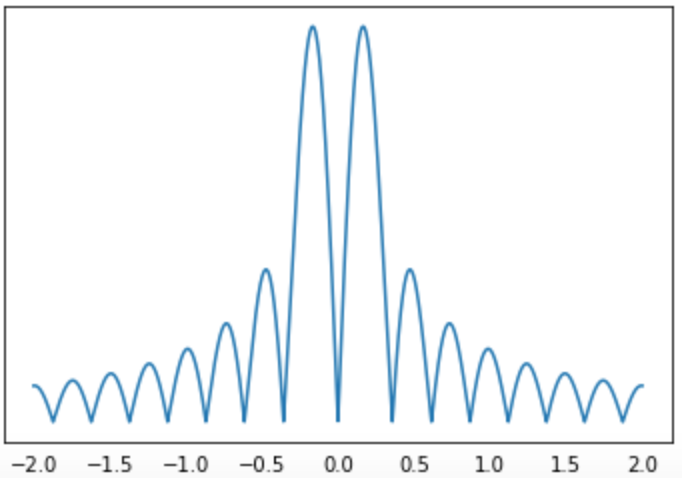
\includegraphics[scale = 1]{2_2.png}
\caption{(b)のスペクトルの絶対値}
\end{figure}
\end{center}

\section*{レポート課題3}
$\displaystyle \sum _{n = -\infty} ^{n=\infty} \delta(t-nT_{0})をフーリエ変換すると、$
\begin{align*}
\int _{-\infty} ^{\infty} \sum _{n = -\infty} ^{n=\infty} \delta(t-nT_{0})e^{-j\omega t}dt &= \sum _{n = -\infty} ^{n=\infty} \int _{-\infty} ^{\infty} \delta(t-nT_{0})e^{-j2\pi f t}dt\\
&= \sum _{n = -\infty} ^{n=\infty} e^{-j2\pi f nT_{0}}
\end{align*}
これは、 $\displaystyle \sum _{n = -\infty} ^{n=\infty} \delta(f-\frac{n}{T_{0}})と等しい、なぜなら、これを逆フーリエ変換すると、$

\begin{align*}
\int _{-\infty} ^{\infty} \sum _{n = -\infty} ^{n=\infty} \delta(f-\frac{n}{T_{0}})e^{-j2\pi f t}df &= \sum _{n = -\infty} ^{n=\infty} \int _{-\infty} ^{\infty} \delta(f-\frac{n}{T_{0}})e^{-j2\pi f t}df\\
&= \sum _{n = -\infty} ^{n=\infty} e^{-j\frac{2\pi n}{T_{0}}t}
\end{align*}
となり、周期$T_{0}$のインパルス列となるから。
\end{document}










